\section{Targets}
\label{sec:ui_targets}

\begin{figure}[H]
    \hspace*{-2.5cm}
    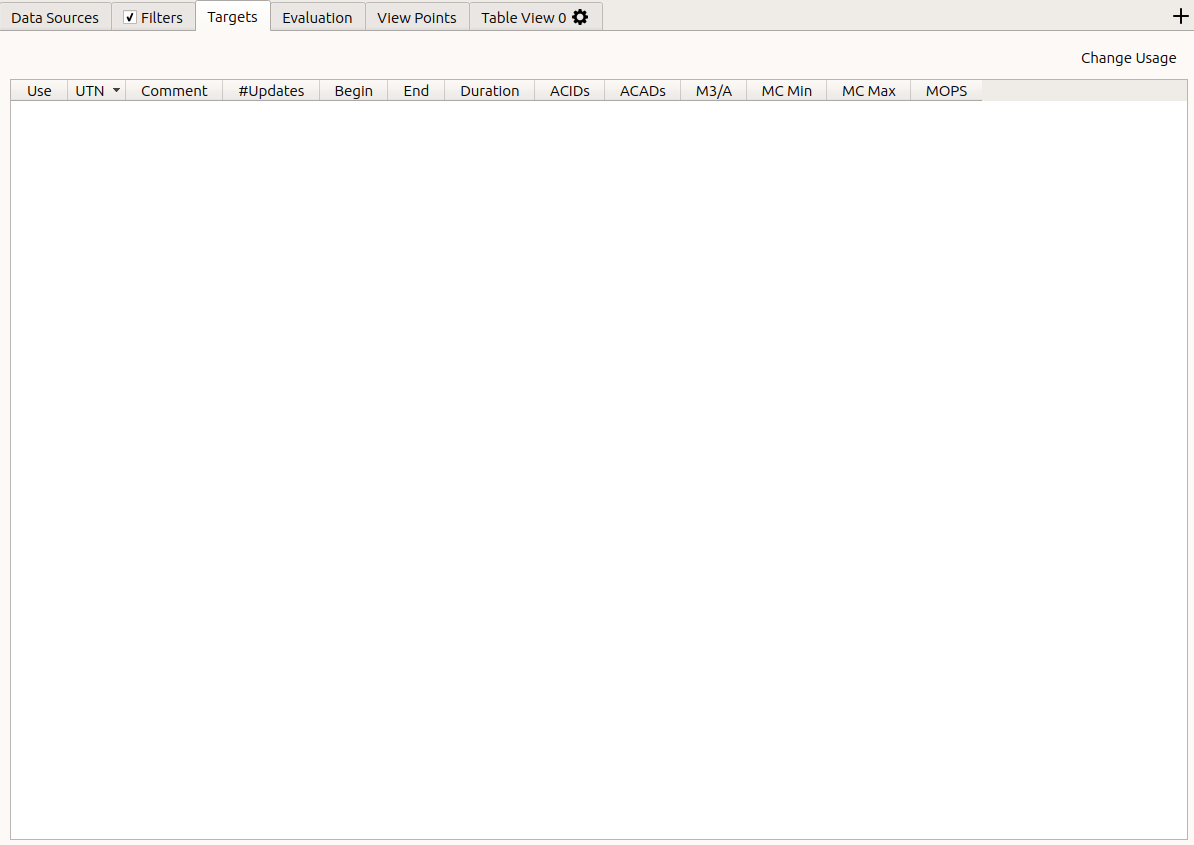
\includegraphics[width=19cm,frame]{figures/ui_targets.png}
  \caption{Targets Overview}
\end{figure}

In this tab, all existing targets are shown. If no associations were calculated, the list is empty. \\

The following columns exist:

\begin{itemize}  
\item Use: Checkbox defining if the target should be used in the evaluation
\item UTN: Unique Target Number
\item Begin: First timestamp of UTN
\item End: Last timestamp of UTN
\item Duration: Duration in HH:MM:SS.SSS
\item \#Updates: Sum number of target reports
\item ACIDs: Target identification(s)
\item ACADs: Target addresses (hexadecimal)
\item M3/A: Mode 3/A code(s) (octal)
\item MC Min: Mode C code minimum [ft]
\item MC Max: Mode C code maximum [ft]
\end{itemize}
\ \\

After running the Calculated Unique Targets task, the table can look as follows:

\begin{figure}[H]
  \hspace*{-2cm}
    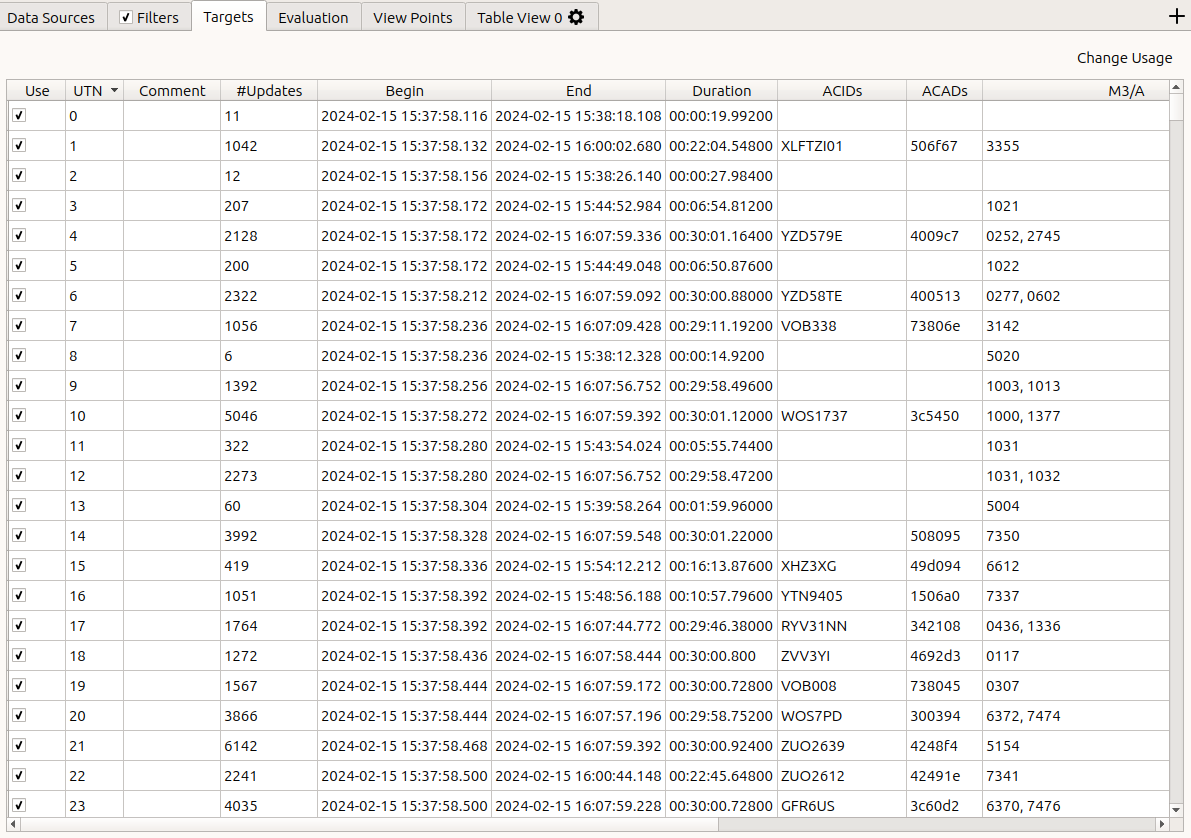
\includegraphics[width=18cm,frame]{figures/ui_targets2.png}
  \caption{Targets Tab with Calculated Unique Targets}
\end{figure}

When clicking a target, all data associated to the respective target is loaded. The Targets tab is useful for inspecting the association results, removing certain targets from evaluations ('Use' checkbox) and inspecting already removed ones. \\

Single rows can be selected by clicking on them which triggers a loading process showing this exact target(s) (with all associated data) in the available Views. Multiple targets can be selected using the shift key (range selection) or control key (add/remove single targets).

\begin{figure}[H]
  \hspace*{-2cm}
    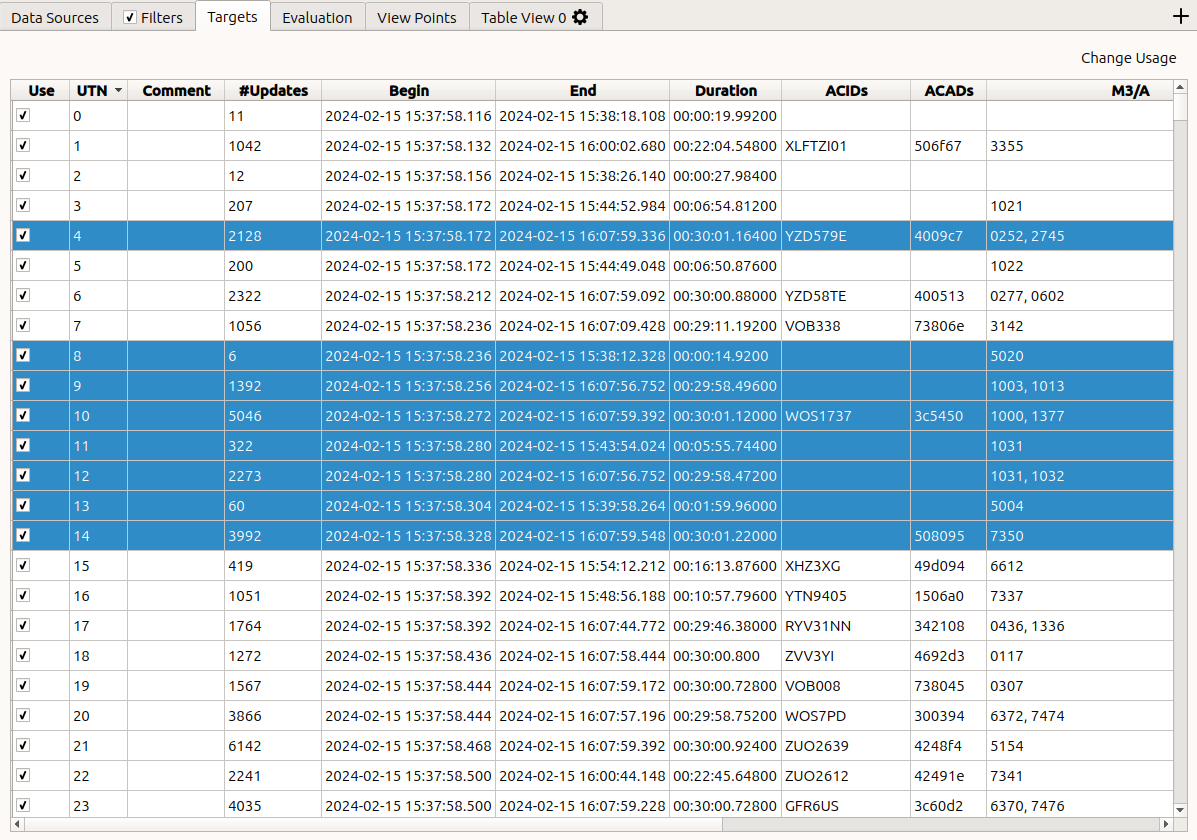
\includegraphics[width=18cm,frame]{figures/ui_targets3.png}
  \caption{Targets Tab with multiple selected targets}
\end{figure}

Please note that such actions can be used at all times during the evaluation and do not require re-loading the evaluation data. \\

Please also note that the target information (including use flag and comment) are persisted in the database.

\subsection{Target Ordering}
\label{sec:ui_target_ordering}

When clicking on a column header, the ordering of the target table can be changed, e.g. to find:

\begin{itemize}  
\item Targets with short duration
\item Missing certain identification attributes
\item Minimum or maximum Mode C code
\end{itemize}
\ \\

Such targets can then be loaded by selecting a range of targets using the shift key - e.g. all with a duration shorter than a certain value of interest.

\subsection{Target Filtering}
\label{sec:ui_target_filtering}

The 'Change Usage' button can be used for the following actions:
\begin{itemize}  
\item Use All: Enable usage for all UTNs
\item Use None: Disable usage for all UTNs
\item Clear Comments: Clear comments of all UTNs
\item Filter: Start 'Filter UTNs' dialog
\end{itemize}
\ \\

The 'Filter UTNs' dialog can be used to dynamically filter UTNs based on the configured values:

\begin{figure}[H]
    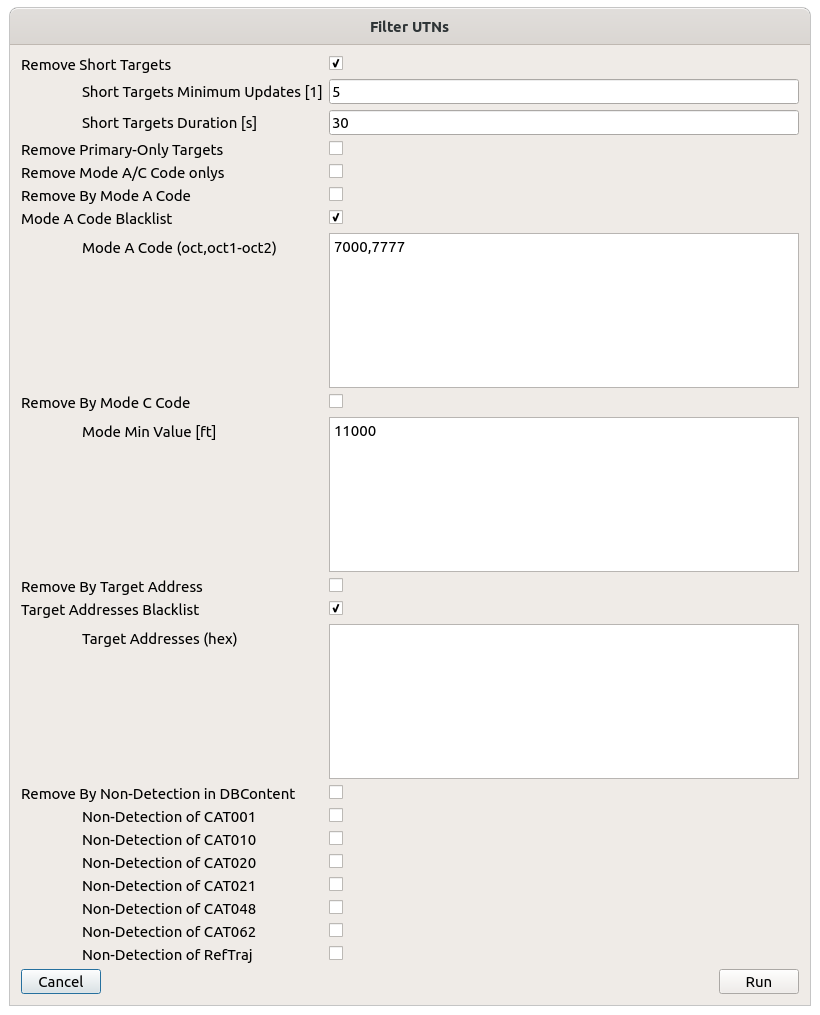
\includegraphics[width=15cm]{figures/filter_utns.png}
  \caption{Targets Filter UTNs dialog}
\end{figure}

\begin{itemize}  
\item Remove Short Targets: Removes targets with a small number of target reports or duration
\item Remove Primary-Only Targets: Removes primary-only targets (w/o secondary attributes)
\item Remove Mode A/C Code onlys: Removes targets without Mode S attributes
\item Remove by Mode A Code: Removes targets having a Mode A code given in the list
\item Mode A Code Blacklist: Whether the Mode A codes should be used as blacklist or whitelist
\item Remove by Mode C Code: Removes targets having a Mode C code smaller than the given value
\item Remove by Target Address: Removes targets having a Mode S target address given in the list
\item Target Address Blacklist: Whether the Target Addresses should be used as blacklist or whitelist
\item Remove by Non-Detection of DBContent: Removes targets not being detected by a given DBContent
\end{itemize}
\ \\

When the 'Run' button is clicked, all (enabled) targets are checked and are disabled if any of the selected filters apply.

\begin{figure}[H]
  \hspace*{-2cm}
    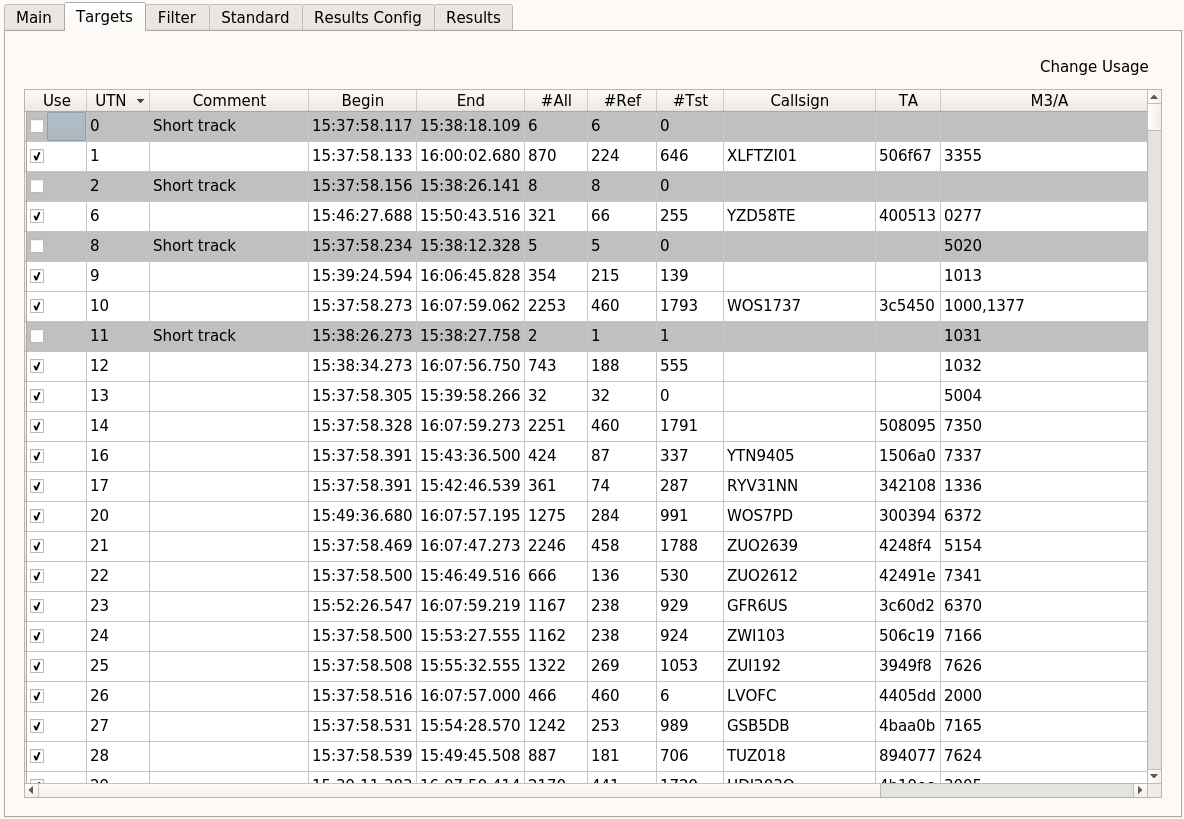
\includegraphics[width=18cm,frame]{figures/filter_utns_done.png}
  \caption{Targets Tab after UTN Filtering}
\end{figure}

Please note that the 'Change Usage' button can be used also after the 'Evaluate' button is used, which automatically updates the evaluation results.
